\documentclass{standalone}
\usepackage{pgfplots}
\pgfplotsset{compat=1.18}

\begin{document}
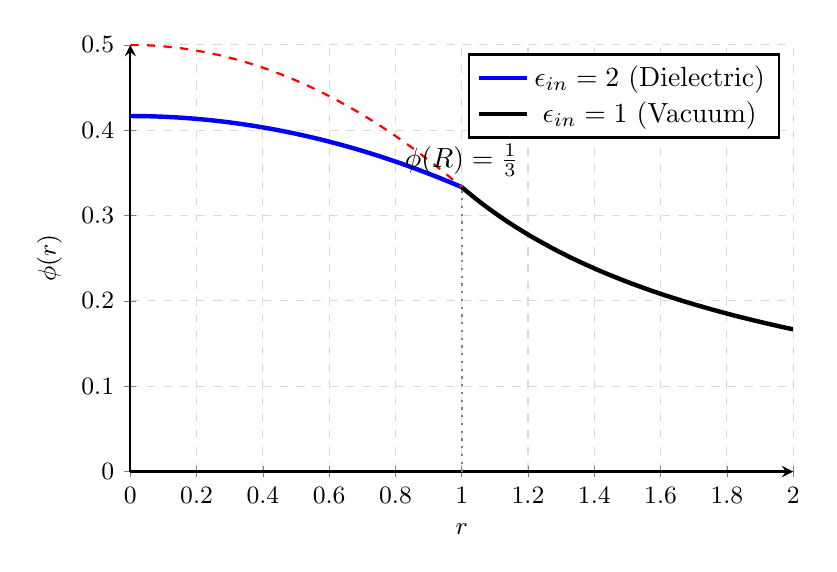
\begin{tikzpicture}
\begin{axis}[
    width=10cm,
    height=7cm,
    xlabel={$r$},
    ylabel={$\phi(r)$},
    xmin=0, xmax=2,
    ymin=0, ymax=0.5,
    domain=0:2,
    grid=major,
    grid style={dashed, gray!30},
    axis lines=left,
    thick,
    tick label style={font=\small},
    label style={font=\small}
]

% Parameters:
% R = 1, rho = 1, eps0 = 1
% eps_in = 2 -> phi_in(r) = (1/3) * [1 + (1/4)*(1 - r^2)] = (1/3)*(1.25 - 0.25*r^2)
% eps_in = 1 -> phi_in_vac(r) = (1/6) * (3 - r^2)
% Outside: phi_out(r) = 1 / (3*r)

% Dielectric case: eps_in = 2
\addplot [domain=0:1, samples=100, blue, ultra thick] {(1/3)*(1.25 - 0.25*x^2)};
\addlegendentry{$\epsilon_{\text{in}} = 2$ (Dielectric)}

% Outside potential (same for both)
\addplot [domain=1:2, samples=100, black, ultra thick] {1/(3*x)};

% Vacuum reference case: eps_in = 1 (dashed)
\addplot [domain=0:1, samples=100, red, thick, dashed] {(1/6)*(3 - x^2)};
\addlegendentry{$\epsilon_{\text{in}} = 1$ (Vacuum)}

% Boundary marker at r = R = 1
\draw[gray, dotted, thick] (axis cs:1,0) -- (axis cs:1,0.3333);
\node[above] at (axis cs:1,0.3333) {$\phi(R) = \frac{1}{3}$};

\end{axis}
\end{tikzpicture}
\end{document}